\chapter{Background} \label{sec:background}

The previous chapter discusses how machine learning algorithms are used to allow computer systems to solve problems that would otherwise be impossible to achieve with traditional programming languages. Artificial neural networks, which are inspired by the neural networks found in living organisms, provide a mechanism to represent solutions to such problems. In this chapter, we take a deeper look at how artificial neural networks are constructed and trained as well as the difficulties and challenges they present.

We begin by describing the artificial neuron (Section \ref{sec:background-artificial-neural-networks-perceptron}), which is the basic building block of artificial neural networks, followed by a description of the gradient descent algorithm, which is used to train these neurons. Then in Section \ref{sec:background-artificial-neural-networks-feed-forward-neural-networks} we explain how we can build more complex models by combining many neurons. In Section \ref{sec:background-deep-learning} we discuss the advantages of deep learning, which involves combining several layers of neurons. Section \ref{sec:background-problem-local-minima} explains the problem of local minima which forms a major challenge to effectively train deep neural networks and which comprises the core of the problem we are solving in this thesis. Finally, in Section \ref{sec:background-sequence-modeling}, we explain recurrent neural networks which are a specialized form of neural networks that allow for modeling of sequential data and which are heavily utilized in the experiments presented in Chapter 4.

\section{Artificial Neural Networks} \label{sec:background-artificial-neural-networks}

The goal of any machine learning system is to learn a function $\hat{f}$ that approximates a target function $f$. In supervised learning, the approximating function might be a classifier of the form $\hat{f}(x) = y$ that learns to map an input vector $\vec{x}$ to a category $\vec{y}$\cite{Goodfellow-et-al-2016}. For example, a system can be made to classify images of handwritten digits into their corresponding values from zero to nine. In this case, when properly learned, the approximate function will accept a vector ($\vec{x}$) that represents the intensities of each pixel in the image and output a vector ($\vec{y}$) representing the class of the image from zero to nine.

There are four components to any machine learning system. First there is the training data from which the learning system acquires the rules that make up the target function, the target function itself, the target function's representation and finally the learning algorithm that updates the representation's parameters to allow the representation to approximate the target function\cite{Mitchell}. Artificial neural networks are one form of target function representation that are inspired by the nervous systems found in living organisms and form the basis of deep learning models.

Artificial neural networks consist of artificial neurons that are mathematical models of a single neuron in a natural nervous system. These artificial neurons accept weighted inputs and produce an output if the sum of the inputs meet a certain threshold. Many neurons can be linked together to form a network. The goal of the learning algorithm is to find a suitable set of weights, which correspond to the synaptic weights found in natural nervous systems, that allow the network to produce the correct output of the function $f(\vec{x})$ given any input $\vec{x}$ in $f$'s domain. That way, the resulting model is said to represent the target function $f$. The remainder of this section provides a detailed look at neural networks and the learning algorithms associated with them.

\subsection{The Perceptron} \label{sec:background-artificial-neural-networks-perceptron}

\begin{figure}[t]
	\centering
	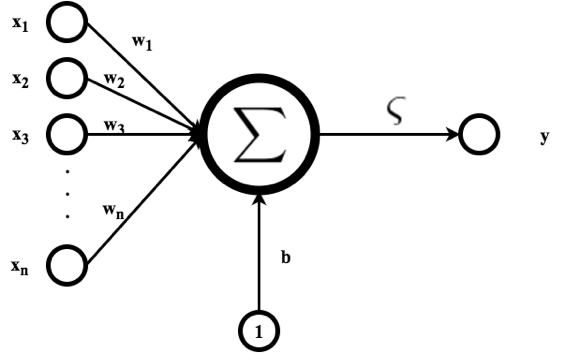
\includegraphics[max width=\textwidth]{perceptron}
	\caption{Visual depiction of a single artificial neuron, sometimes called a perceptron.}
	\label{fig:perceptron}
\end{figure}

Consider the problem of classifying a set of data points into one of several classes. We can reduce this problem to that of finding a decision function $\hat{f}(\vec{x})$ that approximates a true function $f(\vec{x})$, that maps a data point $\vec{x}$ to a class $\vec{y}$. The function $f(\vec{x})$ can be represented as a linear combination of the parameters of $\vec{x}$:
\begin{gather*}
	w_1 x_1 + w_2 x_2 + ... + w_n x_n + b = y_1\\
	w_1 x_1 + w_2 x_2 + ... + w_n x_n + b = y_2\\
	\vdots\\ 
	w_1 x_1 + w_2 x_2 + ... + w_n x_n + b = y_m
\end{gather*}
The problem of learning the decision function then becomes finding a set of weights ($w_1$ to $w_n$ and $b$) that satisfy the provided data points as well as generalize to yet unseen observations\cite{Le15atutorial}.

This system of equations can be depicted as a neuron, like that shown in Figure \ref{fig:perceptron}, that accepts weighted inputs and fires an output that is modified by an activation function. The weights in an artificial neuron resemble synaptic weights found in the neural networks of living organisms. Synaptic weights determine how much influence one neuron has on the next in the network. When considered in the context of artificial neural networks, the weights determine how much the corresponding part of the input affects the output and therefore they act as the medium by which the network is able to represent the decision function\cite{Mitchell}.  

The activation function on the other hand resembles the threshold potential of a natural neural network. It determines how the signal propagates through the system. Likewise, the activation functions of artificial neural networks determine the shape of the output of each unit. Figure \ref{fig:perceptron} shows a neuron with a sigmoid activation. The sigmoid activation function normalizes the output of the unit to a value between zero and one and also produces a non-linear output which is important for some functions\cite{Goodfellow-et-al-2016}.

Once fully trained, the neuron (also called a perceptron) is then used to predict the output of unseen observations using the following formulas:
\begin{gather}
\label{eq:sigmoid}
	z = b + \sum\limits_{i=1}^n x_i w_i\\
	y = \frac{1}{1+e^{-z}}
\end{gather}

\subsubsection{Gradient Descent Algorithm}

The process of discovering the optimum set of weights is performed using the gradient descent algorithm. Gradient descent involves updating the weights of the model in such a way as to minimize the error produced by  applying the training examples to the perceptron relative to the expected target output. The error is depicted as a cost function whose gradient we need to traverse in the negative direction to minimize the error. See Figure \ref{fig:gradient-descent}\cite{Le15atutorial}. The mean square error (MSE) is a popular cost function\cite{Mitchell} given by:
\begin{equation}
E(\vec{w}) = \frac{1}{2} \sum_{d \in D} (t_d - y_d)^2
\end{equation}
where $\vec{w}$ is a vector that comprises the neuron's weights, $D$ is the set of training examples, $t_d$ is the target output for the training example $d$ and $y_d$ is the actual output of the perceptron for training example $d$. 

Figure \ref{fig:gradient-descent} visualizes the error function. Initially the weights are set to random values that place the error at an undesirable level. By iteratively updating the weights, the error is reduced and the weights evolve to capture the decision function. The weight update rule for a linear perceptron where:
\begin{equation}
	y = b + \sum\limits_{i=1}^n x_i w_i\\
\end{equation}
is given by:
\begin{equation}
w_i \leftarrow w_i + \Delta w_i
\end{equation}
where
\begin{equation}
\Delta w_i = -\eta \frac{\partial E}{\partial w_i}
\end{equation}
$\eta$ is the learning rate. The learning rate is a positive value that determines the step size that the gradient descent will take. The larger the learning rate the quicker the descent, however this risks skipping over the optimal weights.

The change $\Delta w_i$ can be obtained by partially differentiating the error with respect to $w_i$:
\begin{equation}
\begin{split}
\frac{\partial E}{\partial w_i} & = \frac{\partial}{\partial w_i} \frac{1}{2} \sum_{d \in D} (t_d - y_d)^2\\
& = \frac{1}{2} \sum_{d \in D} \frac{\partial}{\partial w_i} (t_d - y_d)^2\\
& = \frac{1}{2} \sum_{d \in D} 2(t_d - y_d) \frac{\partial}{\partial w_i} (t_d - y_d) \\
& = \sum_{d \in D} (t_d - y_d) \frac{\partial}{\partial w_i} (t_d - \vec{w}.\vec{x_d}) \\
& = \sum_{d \in D} (t_d - y_d) (-x_{id})
\end{split}
\end{equation}
where $x_{id}$ is the input of training example $d$. The update rule is therefore given by:
\begin{equation} \label{eq:weight-update}
\Delta w_i = \eta \sum_{d \in D} (t_d - y_d) (x_{id})
\end{equation}

\begin{figure}[t]
	\centering
	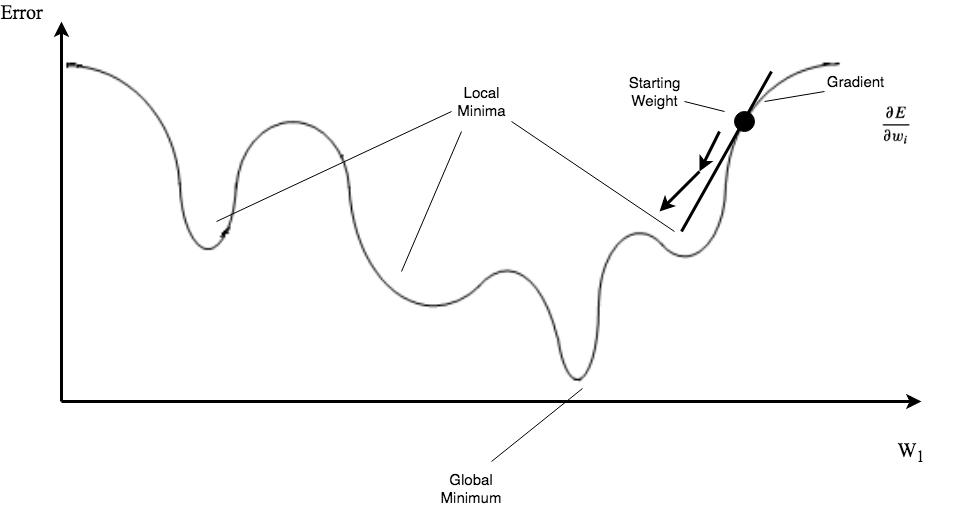
\includegraphics[max width=\textwidth]{gradient-descent}
	\caption{Weights are updated to minimize the error produced by the cost function in an effort to reach the global minimum.}
	\label{fig:gradient-descent}
\end{figure}

\subsubsection{Stochastic Approximation and Batch SGD}

Gradient descent can be considered a strategy for searching through a hypothesis space provided that the error can be differentiated with respect to the hypothesis parameters like the weights of a perceptron. There are two drawbacks however. First, gradient descent tends to be slow in converging on to a local minimum. Second, in more complex hypothesis spaces where there are many local minima, there is no guarantee that the gradient decent will reach the global minimum. There are two ways we can modify the gradient descent algorithm to optimize the learning process: stochastic approximation and batch stochastic gradient descent\cite{Mitchell}.

Instead of running all training examples through the gradient descent algorithm before summing up the error and calculating the weight update, with stochastic gradient descent we calculate the error and perform the weight updates after each training example is introduced to the network. Equation \ref{eq:weight-update} will therefore be replaced by:
\begin{equation}
\Delta w_i = \eta (t_d - y_d) (x_{id})
\end{equation}
This approach can take longer to train a network but has the advantage of adding a stochastic component due to the individual weight changes made for each example. This can increase the likelihood that the algorithm moves out of a local minimum and converges to a more optimal set of weights.\cite{Mitchell}.

A slight modification to the stochastic gradient descent (SGD) approach is to use batch SGD. With batch SGD, instead of updating the weights after every training example, the weights are updated after a batch of examples are introduced to the network. The batch size can vary and can have a significant impact on the training outcome. Using batches of examples maintains some of the speed up of the original gradient descent approach while also retaining the stochastic weight changes that can lead to better models. Batch SGD is used extensively in the experiments presented in Chapter 4.

\subsubsection{Adam Optimizer}

The learning rate is an important hyper parameter that can speed up the learning process when increased. However, higher learning rates can prevent the gradient descent algorithm from reaching a desired minimum in the hypothesis space, especially when the current gradient is close to that desired minimum. One modification that can be made is to introduce a learning rate decay parameter. With learning rate decay, after every epoch (a single iteration where all training examples are introduced to the network) the learning rate is decreased by a factor defined by the decay rate. This makes training faster early in the gradient descent where it is highly unlikely the algorithm will skip a desired minimum and prevents this from happening the closer we converge onto a minimum\cite{Mitchell}.

Other gradient descent techniques introduce a momentum factor to achieve the same goal. This momentum factor prevents the descent algorithm from changing direction too fast. This allows the algorithm to skip smaller shallow local minimums and also to continue down the slope faster when there is no change in gradient\cite{Mitchell}.

Some gradient descent techniques that have grown in popularity over the past decade take learning rate adaptation a step further. The Adam optimizer is one such algorithm that is an extension of the stochastic gradient descent. With Adam optimizer, every weight in the model has its own learning rate. This allows the algorithm to find a solution in a hypothesis space with sparse gradients (where the majority of weights are zero) such as those exhibited by computer vision problems\cite{DBLP:journals/corr/KingmaB14}.

Adam also uses moment to adapt each learning rate based on the current gradient of the parameter in question. Like momentum based techniques, moment allows the algorithm to go down the slope faster when there is little change in the gradient. However, this is done by adapting the learning rate instead of adding an additional factor. Specifically, Adam calculates an exponential moving average for the gradient and the square of the gradient. The learning rate is changed based on these averages and beta1 and beta2 values given as parameters to the optimizer\cite{DBLP:journals/corr/KingmaB14}.  Adam optimizer uses the following parameters with the following recommended values:
\begin{itemize}
	\item Alpha is the initial learning rate and is set to $0.001$
	\item Beta1 the rate by which the exponential moving average is decayed and is set to $0.9$
	\item Beta2 is the rate by which the exponential moving average  of the square of the gradient is decayed and is set to $0.999$
	\item Epsilon is a factor that prevents division by zero  and is usually set to $10^{-8}$
\end{itemize}	

The Adam optimizer is more efficient than other techniques that use a separate learning rate for each parameter. It also allows converging to a solution in the hypothesis space much faster than typical stochastic gradient descent\cite{DBLP:journals/corr/KingmaB14}. For these two reasons, the experiments conducted as part of the research presented in this thesis use the Adam optimizer exclusively as implemented in the TensorFlow library.


\subsection{Feed Forward Neural Networks} \label{sec:background-artificial-neural-networks-feed-forward-neural-networks}

A single neuron is limited to only discovering linear decision functions as show in Figure \ref{fig:separation-surface}(a). However, many real world problems are too complex to be modeled using a linear function (see Figure \ref{fig:separation-surface}(b)). Instead, individual neurons can be combined together into several layers to form a topology known as a feed forward network like the one shown in Figure \ref{fig:feed-forward}. Feed forward networks are composed of one or more fully connected layers, an output layer and zero or more hidden layers\cite{Mitchell}. By increasing the complexity of the network, the number of weights increases and in turn the separation surface (decision function) the model is able to represent also increases in complexity. This allows the neural network to effectively perform more difficult tasks\cite{Bengio07scalinglearning}.

\begin{figure}[t]
	\centering
	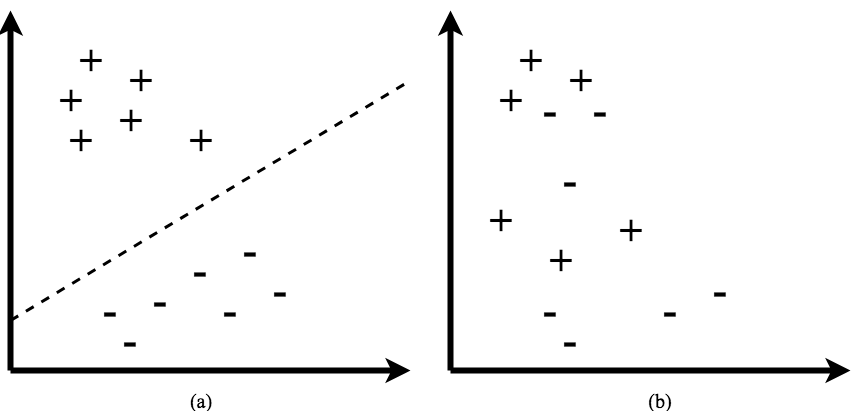
\includegraphics[max width=\textwidth]{separation-surface}
	\caption{A linear decision function (a) can not represent models that can solve more complex problems (b).}
	\label{fig:separation-surface}
\end{figure}

Feed forward networks are trained in the same way as single perceptrons, by running the training dataset through the network and minimizing the error between the outputs and the expected results. Gradient descent is also used to find the approximate weights that will minimize the value of the cost function. However, applying gradient descent to feed forward networks is slightly more involved given the complex nature of the models.\cite{Le15atutorial}.

\begin{figure}[t]
	\centering
	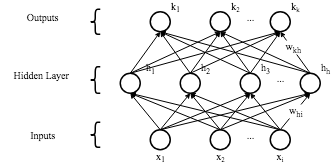
\includegraphics[max width=\textwidth]{feed-forward}
	\caption{A feed forward neural network with a single hidden layer.}
	\label{fig:feed-forward}
\end{figure}

\subsubsection{Backpropagation Algorithm}

The Backpropagation Algorithm is used to apply gradient decent to the individual units of the network\cite{Mitchell}. Initially the network weights are set to random values. Then for each training example, the backpropagation algorithm goes through two stages. First the input is propagated forward and the output $o_u$ of every unit $u$ is calculated. Next comes the backpropagation part where errors are propagated backwards through each layer and new weights are calculated.

For each output unit $k$ an error term $\delta_k$ is calculated
\begin{equation}
\delta_k \leftarrow y_k (1 - y_k)(t_k - y_k)
\end{equation}
where $y_k$ is the actual output of the output unit $k$ and $t_k$ is the target for output unit $k$. Then the error $\delta_h$ for each hidden unit $h$ is calculated
\begin{equation}
\delta_k \leftarrow y_h (1 - y_h) \sum_{k \in outputs} w_{kh} \delta_k
\end{equation}
where $y_h$ is the output from hidden unit $h$ and $w_{kh}$ is the weight of the connection between the hidden unit $h$ and the output unit $k$. Finally the weight of the connection from unit $i$ to unit $j$ is updated using the following update rule
\begin{equation}
w_{ji} \leftarrow w_{ji} + \eta \delta_j x_{ji}
\end{equation}

\subsubsection{Activation Functions}

\begin{figure}[t]
	\centering
	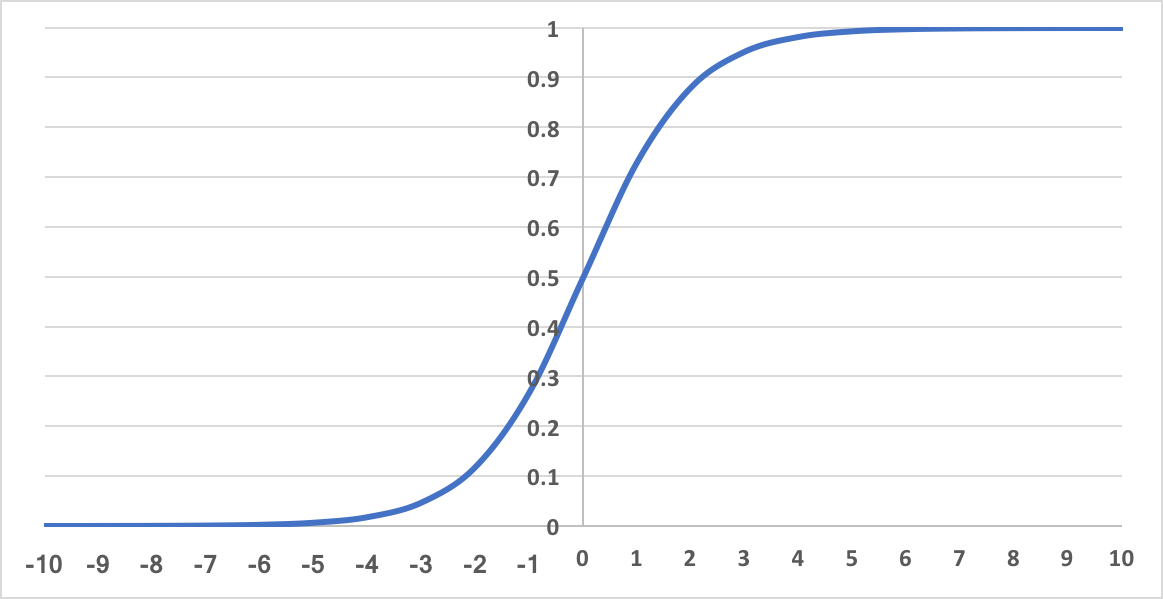
\includegraphics[max width=\textwidth]{sigmoid}
	\caption{A graph depicting the logistic form of the sigmoid function.}
	\label{fig:sigmoid}
\end{figure}

The choice of activation function limits how well the model can represent the underlying problem. In addition, the activation function determines the chain rule that is used to derive the gradient descent update rule. Here we discuss some variations of activation functions and how they affect the ability of neural network models to represent the desired target function. Some functions are best used for output layers because they model a probability distribution like the linear, sigmoid and softmax activations. On the other hand, rectified linear units and hyperbolic tangent activations are used in hidden layers because their derivatives remain generally high. This helps avoid the vanishing gradient problem discussed in Section \ref{sec:background-sequential-models-long-short-term-memory-units}\cite{Goodfellow-et-al-2016}.

Linear units model Gaussian distributions and use a linear activation function where the sum of the weighted inputs is output without transformation. The following formula shows how the output of a linear unit is calculated:
\begin{equation}
\vec{y} = W\vec{x} + b
\end{equation}
Linear activations make it easier for the gradient descent optimizer to find a more desirable minimum. However, they do not represent nonlinear functions very well\cite{Goodfellow-et-al-2016}.

If the output of a neural network involves predicting a binary value, like performing classification with two classes, sigmoid activations can be used. Sigmoid units can be viewed as a linear layer that is then transformed using the sigmoid function\cite{Goodfellow-et-al-2016}. Figure \ref{fig:sigmoid} shows a graph of a sigmoid function and equation \ref{eq:sigmoid} shows the formula for the sigmoid activation function.

The final output activation is known as a softmax activation. These types of units are appropriate for modeling tasks that have an output which is a probability distribution over a discrete variable, for example, a classification problem where the classes are mutually exclusive. Like the sigmoid activation, the softmax activation is a linear layer that is transformed using the softmax function\cite{Goodfellow-et-al-2016}. The following is the softmax function:
\begin{equation}
softmax(z) = \frac{e^z}{\sum{e^z}}
\end{equation}

\begin{figure}[t]
	\centering
	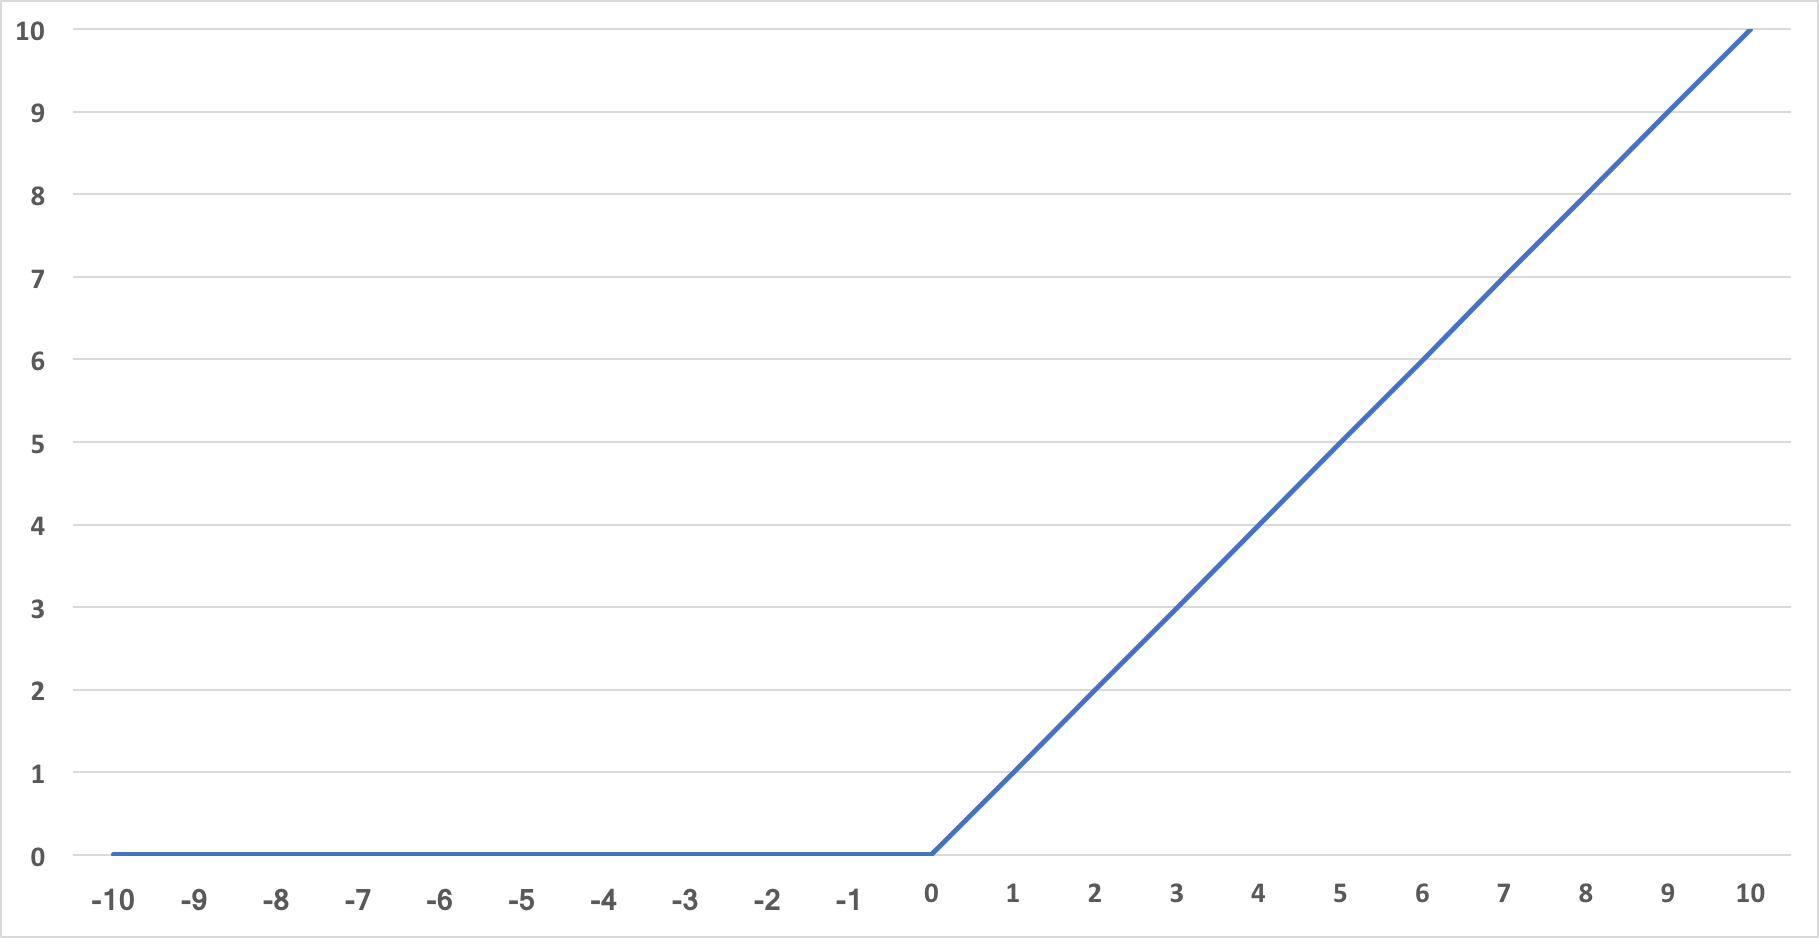
\includegraphics[max width=\textwidth]{relu}
	\caption{A graph of the rectifier function.}
	\label{fig:relu}
\end{figure}

The hyperbolic tangent activation and the rectifier activation are the two most common activation functions in hidden layers. The rectifier is similar to linear activation in that it is easier for gradient descent and also by eliminating values below zero, the gradients remain fairly high which is useful in rapid search for a solution hypothesis \cite{Goodfellow-et-al-2016}. Figure \ref{fig:relu} shows a graph of the rectifier function and the following is the formula for the activation of a rectified linear unit (a neuron with rectifier activation):
\begin{equation}
\label{eq:relu}
y(z) = max\{0, z\}
\end{equation} 

\subsubsection{The Problem of Overfitting}

\begin{figure}[t]
	\centering
	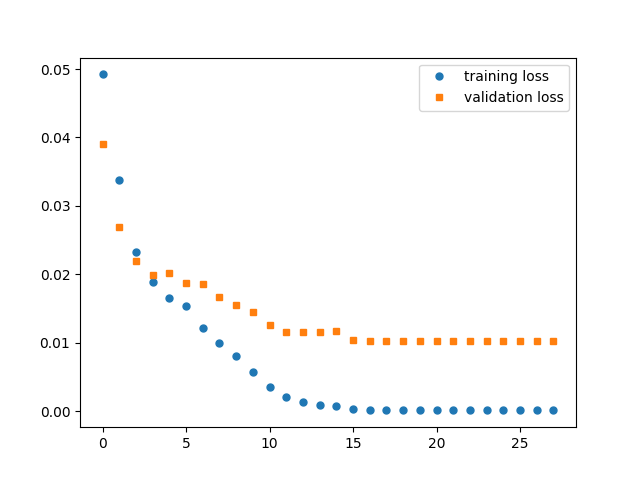
\includegraphics[max width=\textwidth]{overfitting}
	\caption{Comparison of training (circles) and validation (squares) loss over 30 epochs. At the 12th iteration the validation loss stops improving whereas the training loss continues to improve, indicating that the model is starting to overfit.}
	\label{fig:overfitting}
\end{figure}

An important goal of backpropagation is to find a representation that ``fits" the set of training examples and at the same time generalizes to yet unseen data points. Figure \ref{fig:overfitting} shows two graphs that depict the value of the mean squared error against the iteration number of a backpropagation run on a particular dataset. The graph shown in circles shows the errors resulting from the training set and the one in squares shows the errors resulting from the validation set. Notice that the errors from the training set continues to decrease as training proceeds, whereas the errors from the validation set decrease initially but start to stall around the twelfth iteration. This happens because, at the twelfth iteration, the backpropagation algorithm starts to overfit to the training dataset and fails to accurately generalize to the unseen dataset. The weights of the network fit to nuances of the training data that are not representative of the true function. Overfitting is a problem that should be avoided in order for the learning algorithm to create the layers of abstract features that can be used to represent the decision function\cite{Mitchell}.

Using a validation dataset while training is an important mechanism used to prevent backpropagation from overfitting. The validation dataset is independent from the training set and is applied to the model after every epoch. The learning system maintains two copies of the weights of the neural network. One copy holds the weights of the current iteration and the other copy holds the weights of the iteration that performed best on the validation set. When backpropagation stops performing better on the validation set, the best set of weights are returned as the hypothesis learned\cite{Mitchell}.

\subsubsection{K-Fold Cross Validation}

When testing the accuracy of trained neural networks, it is important that the dataset used for testing include a variety of examples that are representative of the overall task. However, with limited datasets, it is difficult to acquire test data that is representative of the problem and therefore it throws into question the effectiveness of the trained model\cite{Goodfellow-et-al-2016}.

Cross-validation is instead used when working with smaller datasets to allow the entire dataset to be used as a test set. With k-fold cross-validation, the dataset is split into k number of non-overlapping subsets. Then training is repeated k times; each time one of the subsets is set aside for testing and the other $k-1$ subsets are used for training. The accuracy score of each iteration is then averaged to produce the overall accuracy of the model. This ensures that the entire dataset contributes to the test set\cite{Goodfellow-et-al-2016}.

In our experiments presented in Chapter 4, we deliberately use small datasets to emulate the difficulty an individual human learner encounters when learning on their own. However, this introduces uncertainty in the accuracy scores obtained from training these models\cite{Goodfellow-et-al-2016}. We therefore use k-fold cross-validation to mitigate this issue.

\subsection{Deep Learning} \label{sec:background-deep-learning}

One of the factors that determines the effectiveness of neural network models is how the features that define the model's inputs and outputs are represented. For example, to construct a model that learns to classify objects in an image, the images would traditionally be pre-processed to extract certain features like edges before being fed into the neural network model. The quality of the feature engineering process significantly affects the outcome of the classification. Certain application domains do not have automated algorithms that can pre-process inputs, in which case feature engineering must be done manually\cite{Goodfellow-et-al-2016}.

To avoid the effort and error introduced by manual feature engineering, machine learning models are adapted to learn feature representations. This usually results in models that perform better than the ones that depended on manually specified features. The ability of these machine learning models to identify the important aspects of the application domain, such as facial recognition, depend on the ability of such models to disentangle the factors of variation that comprise the problem\cite{Bengio:2009:LDA:1658423.1658424}.

This process of separating the important factors from those that are not is considered difficult. In order to capture the complexity of such tasks, we construct representation learning models that are several layers deep. Constructing models in such a layered topology allows the models to represent the application domain in terms of a hierarchy of concepts, with each concept defined through its relation to simpler concepts\cite{Goodfellow-et-al-2016}. Each layer represents the model's understanding of a particular level of abstraction with each level being more abstract than the layer below\cite{Bengio:2009:LDA:1658423.1658424}. This borrows from the fact that our nervous system processes sensory input via a multi-layer hierarchy of neurons\cite{DBLP:journals/corr/abs-1203-2990}. For example, a model that can be used to identify objects in an image can be constructed in several layers. One layer learns to identify edges, the next layer learns to identify simple shapes all the way up to the final layer (output layer) that makes the actual classification.

Figure \ref{fig:feature-representation-learning} shows an example of what the weights of each layer of a deep neural network would learn to represent. Raw pixels are presented as input to the network, the first hidden layer then detects the edges in the image, the second layer detects parts of an object and the final hidden layer detects the object. The model then outputs the classification of what it ``sees" in the input image.

\begin{figure}[t]
	\centering
	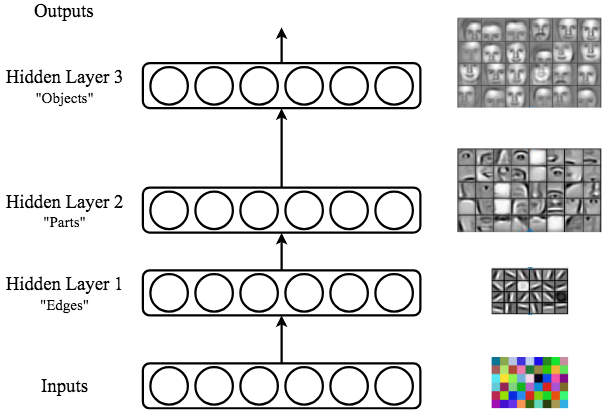
\includegraphics[max width=\textwidth]{feature-representation-learning}
	\caption{Deep feed forward neural network learning to classify objects in an image. Each layer learns to represent a level of abstraction that is more high level than the layer below.}
	\label{fig:feature-representation-learning}
\end{figure}

\subsubsection{The Depth-Breadth Tradeoff}

Besides increasing the representational power of neural network models, empirical evidence also shows that by adding more layers to the neural network architecture the efficiency of the model is also improved. 

The computational complexity of both the feed forward phase and the backpropagation phase of a feed forward neural network is dependent on the number of parameters (weights) that define the model. By having an architecture that is as compact as possible, but at the same time has sufficient complexity to represent the target function, we reduce the required number of weights and therefore have a better performing model.

Bengio 2009 discusses that if a function can be compactly represented by a deep architecture, it might need an exponentially large architecture to be represented by an insufficiently deep one\cite{Bengio:2009:LDA:1658423.1658424}. Therefore, deep architectures help in discovering compact architectures that significantly reduce the computational complexity of the models.

\subsubsection{GPU Training}

The accuracy of trained neural network models depends on the number and variety of the training examples provided. The more factors of variation the problem exhibits the more examples the model will need in order to capture the complexity of the problem. It is therefore important to develop methods to improve the speed of training, especially for difficult problems. One way to accomplish that is by using parallelism. This refers to using more than one processor to train a single model.

There are two forms of parallelizing neural networks. The first is model parallelism, which refers to partitioning the neurons that make up the model onto several processors. Communication is needed so that the outputs of one partition can be fed into another partition. The second type of parallelism is called data parallelism. Each machine holds a copy of the model and the training data is divided among the copies. Each copy is trained independently and then the weight values are integrated after training\cite{Le15atutorial2}.

Many off the shelf computers incorporate Graphics Processing Units (GPUs) that support General Purpose GPU computing (GPGPU). GPUs can have hundreds and sometimes thousands of processing cores collectively allowing for parallel computing. This makes it convenient and affordable to parallelize machine learning. Some machine learning libraries like TensorFlow support running models on GPU powered machines. In this research, we take advantage of GPUs to run our experiments.

\subsubsection{Sequential Models} \label{sec:theory-approach-methodology-sequential-models}

\begin{figure}[t]
	\centering
	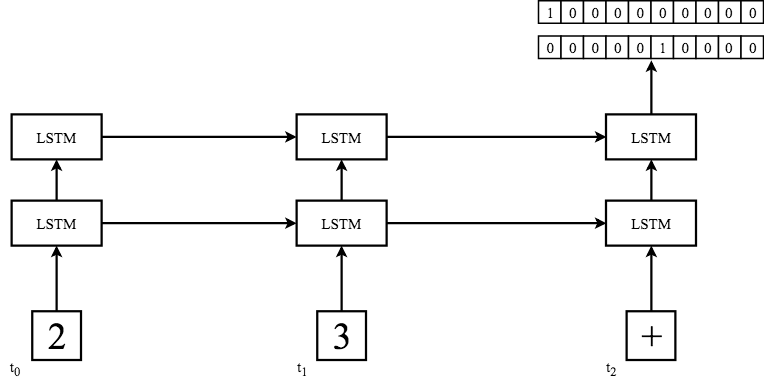
\includegraphics[max width=\textwidth]{sequential-model-arithmetic}
	\caption{A deep LSTM network that accepts a sequence of two operands and learns to perform addition on them.}
	\label{fig:sequential-model-arithmetic}
\end{figure}

When humans perform arithmetic operations, like addition, they tend to read an operand, followed by an operator, followed by another operand and then they perform the operation and produce an output. This approach to arithmetic is sequential in nature and depends on our ability to retain a representation of the operands in our minds as we read them, before we perform the operation. Given that recurrent neural networks are better suited to modeling these kinds of sequential processes, as discussed in Section \ref{sec:background-sequence-modeling}, we therefore opted to using recurrent neural networks for our experiments.

Figure \ref{fig:sequential-model-arithmetic} shows how the arithmetic expression 2 + 3 = 5 can be modeled using recurrent neural networks. On each time step the model accepts a 28x28 image of a handwritten digit from the MNIST dataset. On the last time step the model receives the operator, again in the form of a 28x28 image, and produces an output which is the result of performing the operation on the two operands. The result is represented using a pair of one-hot vectors, one vector represents the least significant digit of the result and the other represents the most significant digit of the result. Notice that we provide the operator on the final time step as opposed to the middle time step. This is because we use reverse Polish notation (RPN) when presenting the operations to the neural networks.

\paragraph{Reverse Polish Notation}

The reverse Polish notation (RPN) is a notation used to depict arithmetic expressions without the need for parentheses to indicate precedence. Unlike traditional mathematical notation where the operands of a binary operator are placed on the left and right of the operator, in RPN both operands precede the operator. The expression
\begin{gather*}
	(7 + 5) - 2
\end{gather*}
would be expressed as
\begin{gather*}
	7\ 5\ +\ 2\ -
\end{gather*}
As long as the operations have a non-variable number of operands, any arbitrarily long sequence of operations can be represented in RPN\cite{wiki:reverse-polish-notation}.

Early stack based computer models based on the work of Dijkstra and Bauer utilized RPN to reduce memory access while evaluating mathematical expressions\cite{wiki:reverse-polish-notation}. Hence, we believe that using RPN to train neural networks to perform arithmetic operations would reduce the complexity of the problem, making it easier to investigate the core hypothesis of this thesis and focus on contrasting the models' accuracy due to the presence of symbols or lack thereof instead of worrying about other factors.

\section{The Problem of Local Minima} \label{sec:background-problem-local-minima}

Combining many layers of features together to form a neural network may increase the expressiveness and accuracy of the model, however, it adds challenges to the training process. A major challenge for the training algorithm is to search for a global minimum in the hypothesis space, given the presence of many local minima in hypothesis spaces with lower dimensions\cite{Larochelle:2009:EST:1577069.1577070} and the presence of many saddle points and plateaus in higher dimensions\cite{DBLP:journals/corr/DauphinPGCGB14}. Figure \ref{fig:gradient-descent} depicts the training set loss as a function of the weights. The complex topology of the feed forward network adds regions in the loss function that act as local minima. In the context of a small dataset, this makes it more likely for the backpropagation algorithm to converge the weights to one of these local minima instead of the desired global minimum\cite{Larochelle:2009:EST:1577069.1577070}. Overcoming this difficulty in training can be achieved by increasing the number of training examples used. Other techniques involve pre-training the network using unsupervised learning first before using the network as a classifier as is the case with deep belief networks\cite{Larochelle:2009:EST:1577069.1577070}.

When comparing machine learning to how we as humans learn, we find that humans also suffer for the presence of effective local minima that hamper their ability to learn from small datasets\cite{Larochelle:2009:EST:1577069.1577070}. In the next chapter, we present our theory that considers how this problem can be overcome in artificial neural networks by introducing a symbolic channel. This symbol channel emulates how the concise knowledge shared by human learners helps individual humans overcome otherwise impoverished training data. The symbolic channel introduces bias that favors regions of the hypothesis space avoiding local minima and allowing the gradient descent process to converge to a more suitable minimum.

\section{Summary} \label{sec:theory-summary}

This chapter presented our basic hypothesis. The theory states that individual human learners struggle to learn new concepts through experimentation alone when the number of examples provided to them is limited. However, through interaction with other learners, common symbols for noisy concepts are shared that allows the learner to overcome the challenges in developing accurate models. We hypothesize that the introduction of such a symbolic channel to an artificial neural network model can also help the model achieve higher levels of accuracy when training with an impoverished dataset.

We also proposed a problem domain to validate this hypothesis, namely to teach artificial neural network models to perform arithmetic on images of handwritten digits. We first explained that the process of learning arithmetic operations can be modeled using sequential neural network architectures. We then presented two methods of supplying symbolic information to these models. Next, two theories were discussed on the role the symbols play in guiding the learning system towards discovering an optimum solution to the problem. Finally, we introduced a new form of symbolic representation, that of temperature encoding, that we believe will capture all aspects of learning to perform arithmetic and will therefore produce the best results. 